\chapter{Expectation Value of the Swap Operator}
\label{swaperator}
%======================================================================

\begin{align}
\langle \SWA \rangle &=
\bra{\Psi_0\otimes\Psi_0}\SWA \ket{\Psi_0\otimes\Psi_0} \\ &= \nonumber
	\left(\sum_{\alpha'_1,\beta'_1}
		\overline{C}_{\alpha'_1,\beta'_1}\sum_{\alpha'_2,\beta'_2} 
		\overline{C}_{\alpha'_2,\beta'_2}
			\big(\bra{\alpha'_1}\bra{\beta'_1}\big)\otimes\big(\bra{\alpha'_2}\bra{\beta'_2}\big)
			  \right) \times \\ 
	& \hspace{4.2cm}
		\left( \sum_{\alpha_1,\beta_1}C_{\alpha_1,\beta_1}\sum_{\alpha_2,\beta_2} 
			C_{\alpha_2,\beta_2}
			\big(\ket{\alpha_2}\ket{\beta_1}\big)\otimes
			\big(\ket{\alpha_1}\ket{\beta_2}\big) \right) \\
	&=\sum_{\alpha'_1,\beta'_1}\sum_{\alpha_1,\beta_1}
		\overline{C}_{\alpha'_1,\beta'_1}C_{\alpha_1,\beta_1}
		\sum_{\alpha'_2,\beta'_2}\sum_{\alpha_2,\beta_2} 
		\overline{C}_{\alpha'_2,\beta'_2}C_{\alpha_2,\beta_2}
		\inn{\alpha'_1}{\alpha_2}\inn{\beta'_1}{\beta_1}
		\inn{\alpha'_2}{\alpha_1}\inn{\beta'_2}{\beta_2} \\
	&=\sum_{\alpha_1,\beta_1} \sum_{\alpha_2,\beta_2}
		\overline{C}_{\alpha_2,\beta_1}C_{\alpha_1,\beta_1}
		\overline{C}_{\alpha_1,\beta_2}C_{\alpha_2,\beta_2}\\
	&= \sum_{\alpha_1,\alpha_2} \left( \sum_{\beta_1}
		 C_{\alpha_1,\beta_1} \overline{C}_{\alpha_2,\beta_1}\right) 
		 \left( \sum_{\beta_2} C_{\alpha_2,\beta_2} \overline{C}_{\alpha_1,\beta_2}\right)
		\label{mmmm}	
\end{align}
We should pause here to work backwards for a bit.
\begin{align}
	\rho_{\rm A} &= {\rm Tr_B} \ket{\Psi_0} \bra{\Psi_0} \\
	&={\rm Tr_B} \left[ \left(\sum_{\alpha_1,\beta_1} 
		C_{\alpha_1,\beta_1}\ket{\alpha_1}\ket{\beta_1}\right)
		\left(\sum_{\alpha_2,\beta_2} 
		\overline{C}_{\alpha_2,\beta_2}\bra{\alpha_2}\bra{\beta_2}\right) \right] \\
	&=   \sum_{\beta_3} \bra{\beta_3} \left[ \left(\sum_{\alpha_1,\beta_1} 
		C_{\alpha_1,\beta_1}\ket{\alpha_1}\ket{\beta_1}\right)
		\left(\sum_{\alpha_2,\beta_2} 
		\overline{C}_{\alpha_2,\beta_2}\bra{\alpha_2}\bra{\beta_2}\right) \right] \ket{\beta_3} \\
	&=   \sum_{\beta_3}  \left[ \left(\sum_{\alpha_1} 
		C_{\alpha_1,\beta_3}\ket{\alpha_1}\right)
		\left(\sum_{\alpha_2} 
		\overline{C}_{\alpha_2,\beta_3}\bra{\alpha_2}\right) \right] 
\end{align}
If we relabel $\beta_3 \rightarrow \beta_1$ and compute a matrix element:
\begin{align}
	\bra{\alpha_1}\rho_{\rm A} \ket{\alpha_2}
	&=   \bra{\alpha_1}\sum_{\beta_1}  \left[ \left(\sum_{\alpha_1} 
		C_{\alpha_1,\beta_1}\ket{\alpha_1}\right)
		\left(\sum_{\alpha_2} 
		\overline{C}_{\alpha_2,\beta_1}\bra{\alpha_2}\right) \right] \ket{\alpha_2} \\
	&= \sum_{\beta_1} C_{\alpha_1,\beta_1} \overline{C}_{\alpha_2,\beta_1} \label{nnnn},
\end{align}
you may notice that \eqref{nnnn} is one of the expressions found in \eqref{mmmm}.
Now we can continue the calculation of $\langle \SWA \rangle$.
\begin{align}
\langle \SWA \rangle &= \sum_{\alpha_1,\alpha_2} \big( \bra{\alpha_1}\rho_{\rm A} \ket{\alpha_2} 
					\bra{\alpha_2}\rho_{\rm A} \ket{\alpha_1}\big) \\
	&= \sum_{\alpha_1} \big( \bra{\alpha_1}\rho_{\rm A} 
				\underbrace{\sum_{\alpha_2} \ket{\alpha_2}\bra{\alpha_2}}_{\mathds{1}}
				\rho_{\rm A} \ket{\alpha_1}\big) \\
	&= \sum_{\alpha_1} \bra{\alpha_1}\rho_{\rm A}^2  \ket{\alpha_1}
\end{align}
\vspace{-5mm}
\begin{align}
	\hspace{-3.3cm}\boxed{\langle \SWA \rangle= {\rm Tr (\rho_A^2)}} \hspace{1cm}
\end{align}

%======================================================================
\chapter{Small-Scale Entropy Calculations}
\label{small}
%======================================================================
\newcommand{\ra}{\rangle}
\newcommand{\la}{\langle}
\newcommand{\ox}{\otimes}
\newcommand{\singlet}[2]{\left( \mid \up_#1 \dw_#2 \ra - \mid \dw_#1 \up_#2 \ra \right) }
\newcommand{\kb}[2]{\mid \! #1 \ra \la #2 \!\mid}

Finding the von Neuman Entanglement Entropy ($S^{\rm vN}$) of a state which is a linear combination (with equal parts) of all vertical and all horizontal valence bonds in a 2x4 site system.
None of the bonds cross the boundary between subsystems A and B.  
The system is illustrated in the diagram below.\\ 

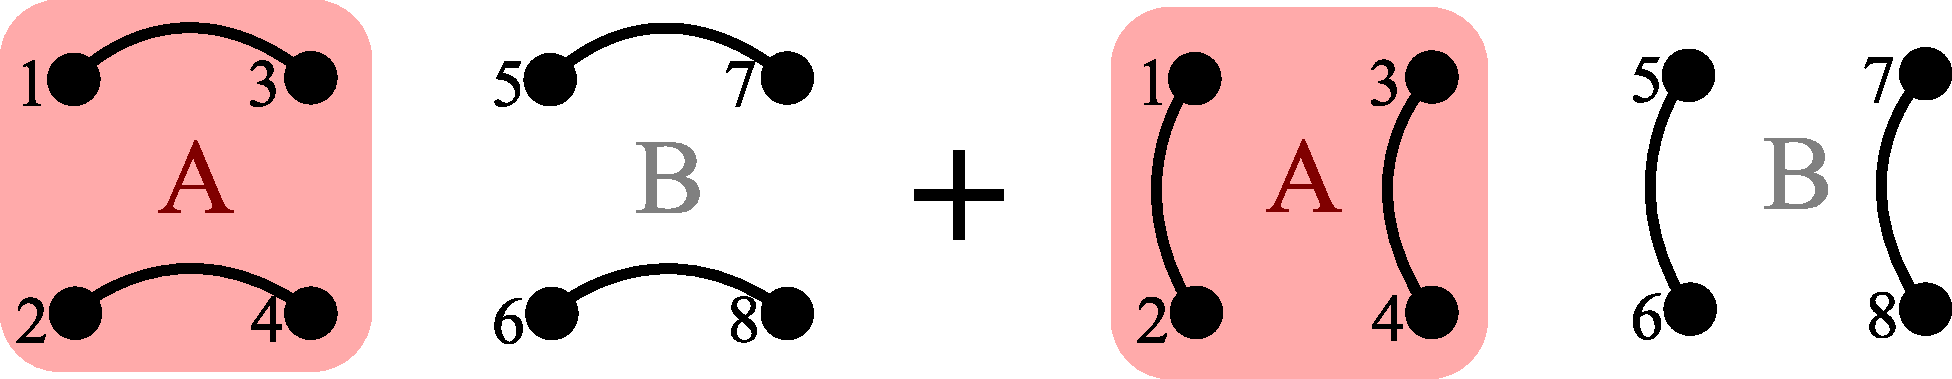
\includegraphics[width=6in]{./figures/made/example2.pdf}

Figure B.1: An equal superposition of two eight-site states.
Region A is the shaded region including sites $1-4$.  
Region B contains the remainder of the sites, $5-8$.
For this state $\VB_{\rm A}=0$ and $\VN_{\rm A}\approx 0.325$.
\\

We start by writing out the wavefunction of the system, where $C$ is the normalization constant.
\begin{eqnarray*}
 \ket{\psi}  &=& C\left[\singlet{1}{2} \ox \singlet{3}{4} \ox \singlet{5}{6} \ox \singlet{7}{8}\right]  \\
	   &     &\;\;\;\;+ C\left[\singlet{1}{3} \ox \singlet{2}{4} \ox \singlet{5}{7} \ox \singlet{6}{8}\right]  \\ 
\end{eqnarray*}
\begin{eqnarray*}
 \ket{\psi}	     &=& C\big[\left(\ket{\up_1\dw_2\up_3\dw_4} - \ket{\up_1\dw_2\dw_3\up_4} -
	              \ket{\dw_1\up_2\up_3\dw_4} + \ket{\dw_1\up_2\dw_3\up_4}\right) \ox \\
	        && \hspace{2in}
	               \left(\ket{\up_5\dw_6\up_7\dw_8} - \ket{\up_5\dw_6\dw_7\up_8} -
	              \ket{\dw_5\up_6\up_7\dw_8} + \ket{\dw_5\up_6\dw_7\up_8}\right)\big]  \\
	     &   +& C\big[\left(\ket{\up_1\up_2\dw_3\dw_4} - \ket{\up_1\dw_2\dw_3\up_4} -
	              \ket{\dw_1\up_2\up_3\dw_4} + \ket{\dw_1\dw_2\up_3\up_4}\right) \ox  \\
	               && \hspace{2in}
	              \left(\ket{\up_5\up_6\dw_7\dw_8} - \ket{\up_5\dw_6\dw_7\up_8} -
	              \ket{\dw_5\up_6\up_7\dw_8} + \ket{\dw_5\dw_6\up_7\up_8}\right)\big] \end{eqnarray*}
\begin{eqnarray*}
 \ket{\psi}	   
	     	&=& C[ \: \ket{\up_1\dw_2\up_3\dw_4} \ox 
	     		\left(\ket{\up_5\dw_6\up_7\dw_8} - \ket{\up_5\dw_6\dw_7\up_8} -
	              	\ket{\dw_5\up_6\up_7\dw_8} + \ket{\dw_5\up_6\dw_7\up_8}\right)  \\
		&& \: + \ket{\up_1\dw_2\dw_3\up_4} \ox
			\left(-\ket{\up_5\dw_6\up_7\dw_8} + \ket{\up_5\dw_6\dw_7\up_8} +
	              	\ket{\dw_5\up_6\up_7\dw_8} - \ket{\dw_5\up_6\dw_7\up_8}\right)  \\
		&& \: + \ket{\dw_1\up_2\up_3\dw_4} \ox
			\left(-\ket{\up_5\dw_6\up_7\dw_8} + \ket{\up_5\dw_6\dw_7\up_8} +
	              	\ket{\dw_5\up_6\up_7\dw_8} - \ket{\dw_5\up_6\dw_7\up_8}\right)  \\
		&& \: + \ket{\dw_1\up_2\dw_3\up_4} \ox
			\left(\ket{\up_5\dw_6\up_7\dw_8} - \ket{\up_5\dw_6\dw_7\up_8} -
			\ket{\dw_5\up_6\up_7\dw_8} + \ket{\dw_5\up_6\dw_7\up_8}\right) \\
		&& \: + \ket{\up_1\up_2\dw_3\dw_4} \ox
			\left(\ket{\up_5\up_6\dw_7\dw_8} - \ket{\up_5\dw_6\dw_7\up_8} -
			\ket{\dw_5\up_6\up_7\dw_8} + \ket{\dw_5\dw_6\up_7\up_8}\right) \\
		&& \: + \ket{\up_1\dw_2\dw_3\up_4} \ox
			\left(-\ket{\up_5\up_6\dw_7\dw_8} + \ket{\up_5\dw_6\dw_7\up_8} +
			\ket{\dw_5\up_6\up_7\dw_8} - \ket{\dw_5\dw_6\up_7\up_8}\right) \\
		&& \: + \ket{\dw_1\up_2\up_3\dw_4} \ox
			\left(-\ket{\up_5\up_6\dw_7\dw_8} + \ket{\up_5\dw_6\dw_7\up_8} +
			\ket{\dw_5\up_6\up_7\dw_8} - \ket{\dw_5\dw_6\up_7\up_8}\right)\\
		&& \: + \ket{\dw_1\dw_2\up_3\up_4} \ox
			\left(\ket{\up_5\up_6\dw_7\dw_8} - \ket{\up_5\dw_6\dw_7\up_8} -
			\ket{\dw_5\up_6\up_7\dw_8} + \ket{\dw_5\dw_6\up_7\up_8}\right)\:] \\ \\			
	     &=& C[ \: \ket{\up_1\dw_2\up_3\dw_4} \ox 
	     		\left(\ket{\up_5\dw_6\up_7\dw_8} - \ket{\up_5\dw_6\dw_7\up_8} -
	              	\ket{\dw_5\up_6\up_7\dw_8} + \ket{\dw_5\up_6\dw_7\up_8}\right)  \\
		&& \: + \ket{\up_1\dw_2\dw_3\up_4} \ox
			(-\ket{\up_5\dw_6\up_7\dw_8} + 2\ket{\up_5\dw_6\dw_7\up_8} +
	             	 2\ket{\dw_5\up_6\up_7\dw_8} - \ket{\dw_5\up_6\dw_7\up_8} \\
		 && \hspace{3.5in}
		 	-\ket{\up_5\up_6\dw_7\dw_8} - \ket{\dw_5\dw_6\up_7\up_8}) \\
		&& \: + \ket{\dw_1\up_2\up_3\dw_4} \ox
			(-\ket{\up_5\dw_6\up_7\dw_8} + 2\ket{\up_5\dw_6\dw_7\up_8} +
	             	 2\ket{\dw_5\up_6\up_7\dw_8} - \ket{\dw_5\up_6\dw_7\up_8} \\
		 &&\hspace{3.5in}
		 	-\ket{\up_5\up_6\dw_7\dw_8} - \ket{\dw_5\dw_6\up_7\up_8}) \\
		&& \: + \ket{\dw_1\up_2\dw_3\up_4} \ox
			\left(\ket{\up_5\dw_6\up_7\dw_8} - \ket{\up_5\dw_6\dw_7\up_8} -
			\ket{\dw_5\up_6\up_7\dw_8} + \ket{\dw_5\up_6\dw_7\up_8}\right) \\
		&& \: + \ket{\up_1\up_2\dw_3\dw_4} \ox
			\left(\ket{\up_5\up_6\dw_7\dw_8} - \ket{\up_5\dw_6\dw_7\up_8} -
			\ket{\dw_5\up_6\up_7\dw_8} + \ket{\dw_5\dw_6\up_7\up_8}\right) \\
		&& \: + \ket{\dw_1\dw_2\up_3\up_4} \ox
			\left(\ket{\up_5\up_6\dw_7\dw_8} - \ket{\up_5\dw_6\dw_7\up_8} -
			\ket{\dw_5\up_6\up_7\dw_8} + \ket{\dw_5\dw_6\up_7\up_8}\right)\:] \end{eqnarray*}
Now we can normalize the state.
\begin{eqnarray*}
\bra{\psi} \psi \ra & = & C^2 \: \: \: = \quad 4 \times ( 1 + 1 + 1 + 1 ) \quad+  
								\quad 2 \times (1 + 4 + 4 + 1 + 1+ 1) \\
				& = & 40
\end{eqnarray*}
For simplicity we relabel the states.
\begin{eqnarray*}
	\ket{a} &=& \ket{\up_5\dw_6\up_7\dw_8}  \qquad  \ket{c} \: \: \: = \quad \ket{\dw_5\up_6\up_7\dw_8} \qquad  \,\ket{e} \: \: \: = \quad\ket{\up_5\up_6\dw_7\dw_8} \\
	\ket{b} &=& \ket{\up_5\dw_6\dw_7\up_8}  \qquad  \ket{d} \: \: \: = \quad \ket{\dw_5\up_6\dw_7\up_8} \qquad  \ket{f} \: \: \: = \quad \ket{\dw_5\dw_6\up_7\up_8} 
\end{eqnarray*}
Now a few steps are skipped as we trace out region A of the system to get the reduced density matrix of region B.
\begin{eqnarray*}
	\rho_{\rm B} &=& {\rm Tr}_A \ket{\psi}\bra{\psi} \\
		&=& \frac{1}{40}\Bigg[ \:2\times \bigg( \ket{a} - \ket{b} -\ket{c} + \ket{d} \bigg)\bigg(\bra{a}-\bra{b}-\bra{c}+\bra{d}\bigg) \\
		&&\quad + \quad
			2\times\bigg( \ket{e} - \ket{b} -\ket{c} + \ket{f} \bigg)\bigg(\bra{e}-\bra{b}-\bra{c}+\bra{f}\bigg) \\
		&&  \quad + \quad 2\times \bigg(\ket{a}-2\ket{b}-2\ket{c}+\ket{d}+\ket{e}+\ket{f}\bigg)
			\bigg(\bra{a}-2\bra{b}-2\bra{c}+\bra{d}+\bra{e}+\bra{f}\bigg)\:\Bigg]
\end{eqnarray*}
\begin{eqnarray*}
	\rho_{\rm B}&=& \frac{1}{20}\Big[\quad\kb{a}{a}-\kb{a}{b}-\kb{a}{c}+\kb{a}{d}\quad-\quad\kb{b}{a}+\,\kb{b}{b}+\,\kb{b}{c}-\,\kb{b}{d} \\
		&&    \quad\:\:\,-\,\kb{c}{a}+\kb{c}{b}+\kb{c}{c}-\,\kb{c}{d} \quad+ \quad \kb{d}{a}-\kb{d}{b}-\kb{d}{c}+\kb{d}{d} \\
		&&    \quad\:\:\,+\,\kb{e}{e}-\kb{e}{b}-\kb{e}{c}+\kb{e}{f} \quad-\quad \kb{b}{e}+\,\kb{b}{b}+\,\kb{b}{c}-\kb{b}{f} \\
		&&    \quad\:\:\,-\kb{c}{e}+\,\kb{c}{b}+\,\kb{c}{c}-\kb{c}{f}\quad+\quad\kb{e}{e}-\,\kb{e}{b}-\kb{e}{c}+\kb{e}{f} \\
		&&    \quad\:\:\,+\kb{a}{a}-2\kb{a}{b}-2\kb{a}{c}+\kb{a}{d}+\kb{a}{e}+\kb{a}{f}   
		\\ &&  \quad\:\:\,- 2\kb{b}{a}+4\kb{b}{b}+4\kb{b}{c}-2\kb{b}{d}-2\kb{b}{e}-2\kb{b}{f} \\
		&&    \quad\:\:\,-2\kb{c}{a}+4\kb{c}{b}+4\kb{c}{c}-2\kb{c}{d}-2\kb{c}{e}-2\kb{c}{f}\\
		&& \quad\:\:\,+\kb{d}{a}-2\kb{d}{b}-2\kb{d}{c}+\kb{d}{d}+\kb{d}{e}+\kb{d}{f} \\
		&&  	\:\quad\:\:\, +\kb{e}{a}-2\kb{e}{b}-2\kb{e}{c}+\kb{e}{d}+\kb{e}{e}+\kb{e}{f}
		\\ && 	\:\quad\:\:\, +\kb{f}{a}-2\kb{f}{b}-2\kb{f}{c}+\kb{f}{d}+\kb{f}{e}+\kb{f}{f} \:\:\Big]
\\ \\
 &=& \frac{1}{20}\Big[\quad\;\;\;2\kb{a}{a} - 3\kb{a}{b} - 3\kb{a}{c} + 2\kb{a}{d} \,\;+\kb{a}{e}\;\, + \kb{a}{f} \qquad\qquad\qquad\qquad\qquad\qquad\qquad\qquad\qquad\qquad 
			\qquad\qquad\qquad\qquad\qquad\qquad\qquad.\\
		&& \qquad  \:\:\:\,- 3\kb{b}{a} +6\kb{b}{b} \,+6\kb{b}{c}-3\kb{b}{d}\, -3\kb{b}{e} -3\kb{b}{f} \\
		&& \qquad  \:\:\:\,- 3\kb{c}{a} +6\kb{c}{b} \,+6\kb{c}{c}-3\kb{c}{d} \,-3\kb{c}{e} -3\kb{c}{f} \\
		&& \qquad  \:\:\:\,+ 2\kb{d}{a} - 3\kb{d}{b} - 3\kb{d}{c} + 2\kb{d}{d} \;\,+\kb{d}{e}\;\, + \kb{d}{f} \\
		&& \qquad  \:\:\:\,+ \;\,\kb{e}{a}\, -3\kb{e}{b} -3\kb{e}{c}\;\:+ \kb{e}{d} + 2\kb{e}{e} \,+ 2\kb{e}{f} \\
		&& \qquad  \:\:\:\,+ \;\,\kb{f}{a} -3\kb{f}{b} -3\kb{f}{c}\:+ \kb{f}{d} + 2\kb{f}{e} + 2\kb{f}{f} \quad\Big] \\ \\ 
		&=& \frac{1}{20}\left[
			\begin {array}{rrrrrr}
			2&-3&-3&2&1&1\\
			\noalign{\medskip}
			-3&6&6&-3&-3&-3 \\ \noalign{\medskip}
			-3&6&6&-3&-3&-3 \\ \noalign{\medskip}
			2&-3&-3&2&1&1 \\ \noalign{\medskip}
			1&-3&-3&1&2&2 \\ \noalign{\medskip}
			1&-3&-3&1&2&2
			\end {array}
			\right]
\end{eqnarray*}
The matrix $\rho_{\rm B}$ was diagonalized using MATLAB.
\begin{eqnarray*}
\rho^{\rm diag}_{\rm B} &=& \frac{1}{10}\left[ \begin {array}{cccccc}
			9&0&0&0&0&0\\
			\noalign{\medskip}
			0&1&0&0&0&0 \\ \noalign{\medskip}
			0&0&0&0&0&0 \\ \noalign{\medskip}
			0&0&0&0&0&0 \\ \noalign{\medskip}
			0&0&0&0&0&0 \\ \noalign{\medskip}
			0&0&0&0&0&0
			\end {array}
			\right] 
			\end{eqnarray*}
We can finally compute the entanglement entropy.
\begin{eqnarray*}
 S^{\rm vN}_{ \rm B} &=& - \rm {\rm Tr}\left(\rho_B{\rm ln} \rho_B\right) =   - {\rm Tr}(\rho^{diag}_B{\rm ln} \rho^{diag}_B) \\ \\ \\
		&=& - {\rm Tr}\left(\left[ \begin {array}{cccccc}
			0.9&0&0&0&0&0\\
			\noalign{\medskip}
			0&0.1&0&0&0&0 \\ \noalign{\medskip}
			0&0&0&0&0&0 \\ \noalign{\medskip}
			0&0&0&0&0&0 \\ \noalign{\medskip}
			0&0&0&0&0&0 \\ \noalign{\medskip}
			0&0&0&0&0&0
			\end {array}
			\right] 
			{\rm ln}\left(\left[ \begin {array}{cccccc}
			0.9&0&0&0&0&0\\
			\noalign{\medskip}
			0&0.1&0&0&0&0 \\ \noalign{\medskip}
			0&0&0&0&0&0 \\ \noalign{\medskip}
			0&0&0&0&0&0 \\ \noalign{\medskip}
			0&0&0&0&0&0 \\ \noalign{\medskip}
			0&0&0&0&0&0
			\end {array}
			\right] \right)\right) \\ \\ \\
		&=& -0.9{\rm ln}(0.9) - 0.1{\rm ln}(0.1) \approx 0.325 \neq S^{\rm VB}_{\rm B} = 0
\end{eqnarray*}


